\subsection{External Receipt Text}
\label{sec:eval:external_receipts}

We use SROIE receipt transcriptions and human key-information labels
\citep{ref_sroie2019} to test repair outside the Chinese record collections.
A fixed random sample contains 60 of the 626 documents in the
community-corrected trainval mirror (seed 20260922). Text lines are joined
in their stored order. The model receives this text and the four field
names: company, date, address, and total. Field values are read separately
by the scorer. One receipt lacks an address annotation, giving 239 evaluated
fields; the missing annotation is excluded from scoring for every method.
All four fields remain available to the model.

A Gemma call first extracts each graph. The three repair contexts then
receive the same extracted graph, using the settings in
Section~\ref{sec:impl:enhancement}. Sampling and settings were fixed before
inference. This gives 60 extraction calls and 180 repair outcomes, each of
which is scored before and after filtering. We reuse the source-copy and
structural baselines without receipt-specific tuning. The primary score
uses exact triple matching. A secondary score ignores case and whitespace
in field values to separate these formatting differences from other errors.

\begin{table*}[t]
\centering
\caption{External SROIE results on 60 receipt transcripts. Exact match is over
annotated fields. Normalized F1 ignores case and whitespace in values.}
\label{tab:external_receipts}
\small
\begin{tabular}{lrrrr}
\toprule
Method & Triple F1 & Exact match & Normalized F1 & Preservation \\
\midrule
Extracted input & 0.7944 & 0.3333 & 0.8153 & 1.0000 \\
Rule Only & 0.7944 & 0.3333 & 0.8153 & 1.0000 \\
Source-field Copy & 0.0000 & 0.0000 & 0.0000 & 0.0000 \\
Base, raw & 0.7944 & 0.3333 & 0.8153 & 1.0000 \\
Base, gate & 0.7915 & 0.3333 & 0.8123 & 0.9944 \\
Diagnostic, raw & 0.7944 & 0.3333 & 0.8153 & 1.0000 \\
Diagnostic, gate & 0.7915 & 0.3333 & 0.8123 & 0.9944 \\
SHACL context, raw & 0.7986 & 0.3333 & 0.8194 & 1.0000 \\
SHACL context, gate & 0.7956 & 0.3333 & 0.8165 & 0.9944 \\
\bottomrule
\end{tabular}
\end{table*}

The extracted graphs reach 79.44\% F1.
After filtering, base, diagnostic, and SHACL contexts reach
79.15\%, 79.15\%, and 79.56\%, respectively
(Table~\ref{tab:external_receipts}). The diagnostic--base difference is
$0.00$ points (95\% CI: $[0.00, 0.00]$;
paired randomization $p=1.0000$).
The field-copy parser reaches 0.00\% F1 on these transcripts,
compared with 100\% on the serialized records.

Of the 239 reference values, 220 occur literally in the transcripts.
The other 19 values are absent as exact source strings.
Across the 180 repair responses, filtering rejects 3 candidate occurrences,
all matching a reference value. They concern the same address in three arms:
the source contains a double space, while the JSON parser collapses candidate
whitespace. A post-run check applies the same whitespace normalization to the
source and retains this address in all three arms. With the original responses,
F1 becomes 79.44\% for base and diagnostic contexts
and 79.86\% for SHACL context; exact graph
match remains 33.33\%. The main table keeps the fixed
protocol results, and the separate check identifies the effect of this
normalization mismatch.

The run contains 240 recorded requests,
including retries, and 240 successfully parsed outcomes.
Mean repair request times are 7.87,
7.92, and 8.05 seconds
for base, diagnostic, and SHACL contexts. Their mean input lengths are
661, 715, and
2276 tokens. These times include
request pacing and exclude shared extraction and context preparation.

\begin{figure}[t]
\centering
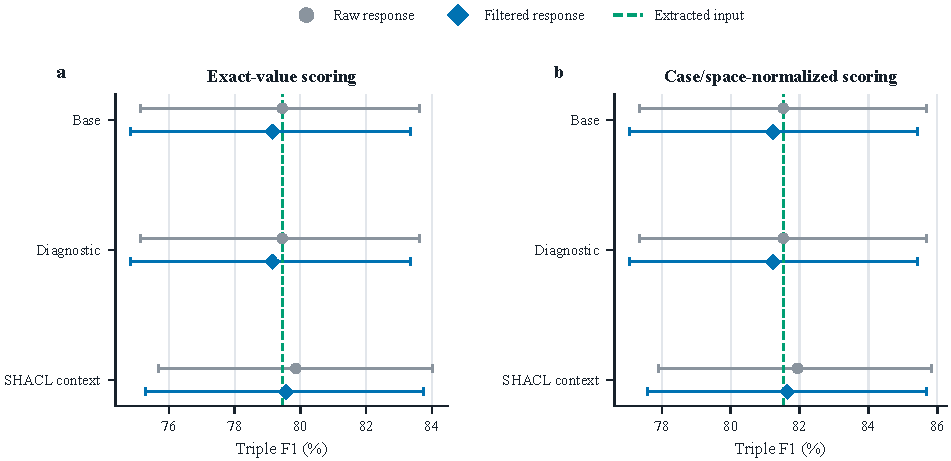
\includegraphics[width=0.98\textwidth]{figure/experiments/external_receipts.pdf}
\caption{Repair on independent receipt text. Points show mean triple F1 and
95\% document-bootstrap intervals. Raw and gated results share model responses;
the dashed line marks the extracted input.}
\label{fig:external_receipts}
\end{figure}
